%% LyX 2.2.1 created this file.  For more info, see http://www.lyx.org/.
%% Do not edit unless you really know what you are doing.
\documentclass[12pt,english]{article}
\usepackage{charter}
\usepackage[T1]{fontenc}
\usepackage[latin9]{inputenc}
\usepackage{graphicx}
\usepackage{setspace}
\usepackage[authoryear]{natbib}
\doublespacing

\makeatletter

%%%%%%%%%%%%%%%%%%%%%%%%%%%%%% LyX specific LaTeX commands.
%% Because html converters don't know tabularnewline
\providecommand{\tabularnewline}{\\}

%%%%%%%%%%%%%%%%%%%%%%%%%%%%%% User specified LaTeX commands.
\usepackage[hmargin=2.5cm,vmargin=2.5cm]{geometry}
\usepackage{layout}
\usepackage{indentfirst}

\makeatother

\usepackage{babel}
\begin{document}

\title{About Those Lab Reports: A Guide to Formatting}

\author{Anneya Golob}

\date{January, 2016}
\maketitle

\part*{Abstract }

This is where you should write a quick summary of your experiment
and most interesting results. In the real world, the \textbf{Abstract}
(and probably\textbf{ Conclusions} too) will often be the only section
people read so it's important to make it concise and pack a powerful
scientific punch. Think of it as a trailer full of spoilers for a
movie so incredibly awesome that you still want to pay money to see
the whole thing. If you have numerical results it's a good idea to
include them.

As an example, here is the abstract from \citet{pmid16007907}:

\begin{center}
\begin{minipage}[t]{0.9\textwidth}%
\begin{singlespace}
\textit{\small{}The typical spices used in winter include nutmeg,
cinnamon, clove and anise. These spices contain two groups of chemicals,
the allylbenzenes and their isomers, the propenylbenzenes. It was
suggested 40 years ago by Alexander Shulgin that these substances
act as metabolic precursors of amphetamines. The biotransformation
of these precursors to nitrogen-containing metabolites is reviewed.
These reactions have not been reported in humans. Whether or not the
pharmacology and toxicology of spices such as nutmeg can be explained
on the basis of their allylbenzene or propenylbenzene content is speculative.
Humans may be exposed to amphetamines derived from these precursors
in forno, the formation during baking and cooking, for example in
the preparation of Lebkuchen, or Christmas gingerbread. It is possible
that this may be responsible, in part, for uplifting our mood in winter.
However, the role of these aromatic substances, acting simply as odours,
evoking old memories of winters past, cannot be ignored. Whether spices
have a true pharmacological effect or they act as aromatherapy remains
to be elucidated through clinical and laboratory studies.}
\end{singlespace}
%
\end{minipage}
\par\end{center}

\section{Theory/Introduction}

\begin{singlespace}
In this section you want to summarize the history of the field that
motivated your particular experiment and explain the basic theory
you use to design the procedure and interpret the results. Include
references where appropriate. 

As an example, here is the introduction from \citet{2012PhRvL.108g8101G}:


\end{singlespace}\begin{center}
\begin{minipage}[t]{0.8\textwidth}%
\begin{singlespace}
\textit{\small{}One of the most familiar features of a bundle of hair
such as a ponytail is its `body' or `volume.' Close examination reveals
that this property arises in a subtle way from the stiffness and shapes
of the individual fibers, whose meandering paths through the bundle
produce many collisions with other hairs. These meanderings are in
part a consequence of the contacts themselves, but hairs also have
an intrinsic waviness or curliness. Such curvatures may be generated
during growth, and vary with ethnicity. They are clearly also modied
by chemical, thermal, and mechanical forces, as in the `water wave'
treatment, or a `perm'. From Leonardo to the Brothers Grimm our fascination
with hair has endured in art and science. Yet, we still do not have
an answer to perhaps the simplest question that captures the competing
eects of lament elasticity, gravity, and mutual interactions: }\textsl{\small{}What
is the shape of a ponytail?}\textit{\small{} Note that the average
human has $10^{5}$ head hairs, so if even a modest fraction is gathered
into a ponytail, the number involved is enormous: this is a problem
in statistical physics.}
\end{singlespace}
%
\end{minipage}
\par\end{center}

At this point, you might want to include equations to clearly explain
the theory behind your procedure. Later in their paper, \citet{2012PhRvL.108g8101G}
describe the equation of state (EOS)\footnote{It's fine if you use abbreviations or initialisms in your document
as long as you define them the first time they're used. } of the ponytail using their proposed definition of the energy of
an axisymmetric bundle of hair fibers:

\begin{equation}
\varepsilon\left[\rho,{\bf {t}}\right]=d^{3}\mathrm{{\bf {r}}}\rho\left(\frac{1}{2}A\kappa^{2}+\varphi({\bf {r}})+\left\langle u\right\rangle \right),\label{eq:pony}
\end{equation}

where $\kappa=\left|\left({\bf t\cdot{\bf \nabla}}\right){\bf t}\right|$
is the curvature field. The terms in Eqn. \ref{eq:pony} are the elastic
energy of mean curvature, the bending modulus $A$, the external (
e.g. gravitational) potential $\varphi$, and a fiber connement energy
per unit length $\left\langle u\right\rangle $ that aggregates all
terms involving disorder, such as contacts and natural curvatures. 

Notice that the equation is centered, numbered and because it's part
of the sentence, includes punctuation where appropriate. Most word
processors are capable of automatically dealing with equation formatting.
If you want to continue in upper year science courses and beyond,
you'll want to start using \LaTeX{} to format your documents sometime
soon.

\section{Apparatus \& Procedure}

This is where you talk about what physical stuff and/or software you
used in your experiment and how you used it. This section should \textbf{not}
include your results. Your goal here is to explain everything thoroughly
enough for a reader to know how to precisely reproduce your procedure.
To accomplish this, you'll want to include every tiny detail that
might be relevant while taking care to state things plainly and be
as concise as possible.

Feel free to add figures or tables that enhance and clarify the explanations
you provide in writing. Note that all figures and tables require a
caption. These are easy to add in \LaTeX{} and most word processors.
Make sure that all figures you include get mentioned in the text.

\begin{figure}
\begin{centering}
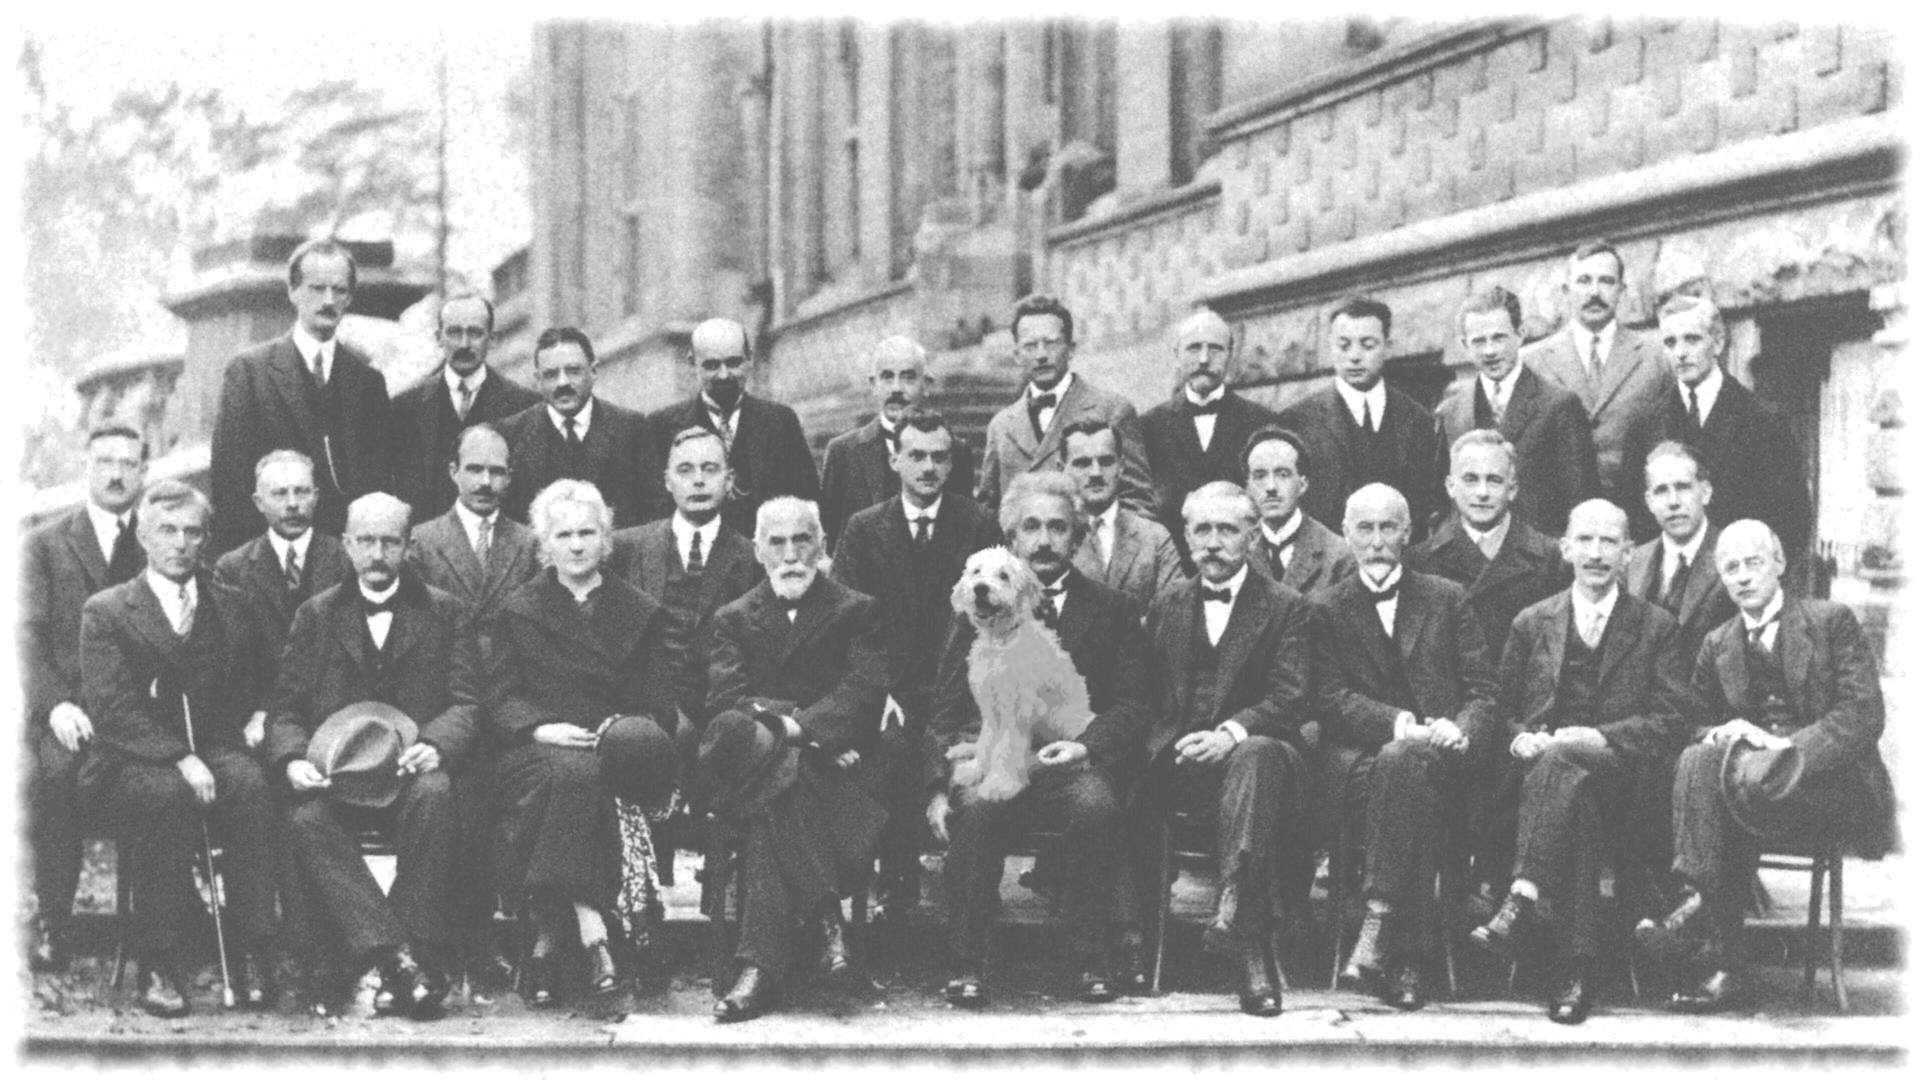
\includegraphics[width=0.8\textwidth]{solvay}
\par\end{centering}
\caption{\label{fig:ras}This is a picture of my dog, Rasalhague, attending
the 1927 Solvay International Conference on Electrons and Photons.
You'll probably want to include figures that show more circuit diagrams
and fewer dogs, but dogs are always welcome. }
\end{figure}

\begin{table}
\begin{centering}
\begin{tabular}{|r|c|}
\hline 
\textbf{Item} & \textbf{Known Occurences}\tabularnewline
\hline 
\hline 
Hat & 1\tabularnewline
\hline 
Everyday sock & 3\tabularnewline
\hline 
Pair of soccer socks & 1\tabularnewline
\hline 
Wrapped granola bar & 1\tabularnewline
\hline 
Dirty Kleenex & 600\tabularnewline
\hline 
Stick & 300\tabularnewline
\hline 
Bowl of dog food & $3284$\tabularnewline
\hline 
Danaerys Targaryen keychain & 1\tabularnewline
\hline 
Platter of smoked salmon & 1\tabularnewline
\hline 
\end{tabular}\caption{\label{tab:stuffrasate}Stuff my dog (see Figure \ref{fig:ras}) ate.}
\par\end{centering}
\end{table}


\subsection{A Subsection}

You can add subsections to organize the content of your report.

\section{Data \& Analysis}

Now that you've described the finicky details of your procedure, it's
time to talk about the data it yielded and what you did with them.
Describe any statistical methods you used to understand your data
and state all of your numerical results. Show off all the plots you
made with figures, as described in Section 2. You can always refer
to things you've labelled in the document, like Fig. \ref{fig:ras},
Equation \ref{eq:pony}, and Table \ref{tab:stuffrasate}. 

The PHYS 2400 lab manual includes specific Analysis Questions throughout.
They should serve as prompts for things that you'll definitely want
to touch on as you explain your analysis and results (some of these
points might belong in the Results and Discussion section, you can
go ahead and put them there if it feels right.) These points should
come up organically as you write, but I'm sure Sam will appreciate
if you point out places where you're answering a question posed in
the manual using footnotes\footnote{This is a footnote. It's easy to format using \LaTeX{} or your WYSIWYG
word processor of choice.}.

\section{Results \& Discussion}

Here, you need to summarize the results of your analysis and interpret
them. Is there anything weird going on? Talk about how accurate your
results are and what you could do to improve accuracy and minimize
uncertainty. Discuss the implications of what you've found on the
field and what should be considered next, science-wise, to advance
the state of human knowledge, explore the phenomenon more deeply etc.

\section{Conclusions}

Like I said in the Abstract, there's a good chance that this is one
of the only things people might read (fortunately for you, we'll pore
over every word of your lab reports in order to grade you fairly)
so you need to make it count! Summarize your important results (again),
figure out what final conclusions you can draw from them and how these
conclusions fit into the related science that's been done by other
people (and maybe you!) 

Science Achieved.

\begin{singlespace}
\bibliographystyle{aa}
\addcontentsline{toc}{section}{\refname}\bibliography{format}

\end{singlespace}

\appendix

\section*{Appendices}

\section{Sample Calculations}

Here, we'll want to see examples of all the non-trivial calculations
you made during the lab and derivations used to propagate uncertainties.
\end{document}
